\documentclass[polish, twoside, 12pt]{mwart}
\usepackage[polish]{babel}
\usepackage{polski}
\usepackage[T1]{fontenc}
\usepackage[utf8]{inputenc}

\usepackage{graphicx}
\graphicspath{ {../figures/} }

\let\stdsection\section
\renewcommand*{\section}{\clearpage\stdsection}
\emergencystretch=3em
\linespread{1.1}

\author{Kewin Polok}
\title{Praca dyplomowa magisterska}

\begin{document}

\maketitle
 
\newpage

\tableofcontents

\newpage

\listoffigures
 
\listoftables

\newpage

\section{Wstęp}

\subsection{Cel pracy}

\subsection{Układ pracy}

\section{Specyfikacja problemu}

\subsection{Założenia dotyczące problemu}

\section{Przeglądarka internetowa}

Przeglądarka internetowa (ang. \emph{web browser}) to program komputerowy służący do pobierania i wyświetlania stron internetowych udostępnianych przez serwery WWW. Komunikacja z serwerem odbywa się najczęściej za pomocą protokołu HTTP (ang. \emph{Hypertext Transfer Protocol})lub odpowiednika w wersji szyfrowanej HTTPS (ang. \emph{Hypertext Transfer Protocol Secure}). Nierzadko przeglądarki internetowe są w stanie obsługiwać inne protokoły takie jak np. FTP (ang. \emph{File Transfer Protocol}) wykorzystywany do serwerów plików, czy też protokoły POP3 (ang. \emph{Post Office Protocol}), IMAP (ang. \emph{Internet Message Access Protocol}) i SMTP (ang. \emph{Simple Mail Transfer Protocol}) wykorzystywane do poczty elektronicznej. 

\begin{figure}[ht]
    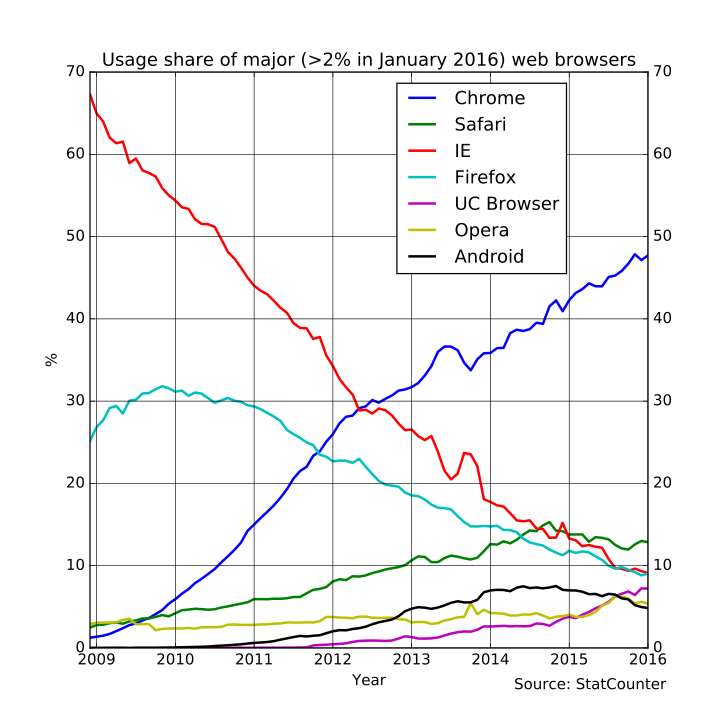
\includegraphics[width=\textwidth]{web-browers-usage-share.png}
	\caption{Udział najwaznieższych przeglądarek na rynku w latach 2009-2016}
	\label{figure1}
\end{figure}

\subsection{Najważniejsze technologie}

Współczesna przeglądarka cechuje się bardzo dobrą obsługą następujących technologii:

\begin{itemize}
\item HTML 5 (ang. \emph{Hypertext Transfer Protocol})
\item CSS 3 (ang. \emph{Cascading Style Sheets})
\item JavaScript
\item DOM (ang.\emph{Document Object Model})
\item CSSOM (ang.\emph{Cascading Style Sheets Object Model})
\end{itemize}

\subsection{Ładowanie strony internetowej}

\subsection{Model współbieżności oraz Event loop}

\subsection{Cykl życia zasobu}

\section{Biblioteka do badań}

\section{Biblioteki programistyczne}

\subsection{Angular 1}

\subsubsection{Opis}

\subsubsection{Wady i zalety}

\subsubsection{Mechanizm działania}

\subsubsection{Implementacja}

\subsection{Angular 2}

\subsubsection{Opis}

\subsubsection{Wady i zalety}

\subsubsection{Mechanizm działania}

\subsubsection{Implementacja}

\subsection{React}

\subsubsection{Opis}

\subsubsection{Wady i zalety}

\subsubsection{Mechanizm działania}

\subsubsection{Implementacja}

\subsection{Vue.js}

\subsubsection{Opis}

\subsubsection{Wady i zalety}

\subsubsection{Mechanizm działania}

\subsubsection{Implementacja}

\subsection{Mithril.js}

\subsubsection{Opis}

\subsubsection{Wady i zalety}

\subsubsection{Mechanizm działania}

\subsubsection{Implementacja}

\subsection{Porównanie bibliotek}

\section{Badania wydajnościowe}

\subsection{Badania wydajności pamięciowej}

\subsection{Badania wydajności czasowej}

\section{Porównanie wyników i wnioski}

\section{Podsumowanie}

\subsection{Dalszy rozwój}

\end{document}